\documentclass[MachineLearning]{subfiles}
\begin{document}

%@@@@@@@@@@@@@@@@@@@@@@@@@@@@@@
% summarizes lecture 3
% author: Benjamin Ellenberger

\section{Regression}
In statistics, regression analysis is a statistical process for estimating the relationships among variables (one independent variable Y and one or more independent variable (\(X_1,\ldots,X_d\))). More specifically, regression analysis helps one understand how the typical value of the dependent variable (or 'criterion variable') changes when any one of the independent variables is varied, while the other independent variables are held fixed. A model of the relationship is hypothesized, and estimates of the parameter values are used to develop an estimated regression equation. Various tests are then employed to determine if the model is satisfactory.If the model is deemed satisfactory, the estimated regression equation can be used to predict the value of the dependent variable given values for the independent variables. (Source: Wikipedia and Encyclopedia Britannica on Regression)\\
\begin{itemize}
\item Object space \(\mathcal{O}\)
\item Measurement/Feature space \(\mathcal{F} = \R^d \times \R\)
\item Data \(\mathcal{Z} = \{(x_i,y_i) \in \R^d \times \R : 1 \geq i \geq n\}\)
\end{itemize}
\textbf{The problem of regression}: What is the optimal estimate of a function \(f: \R^d \rightarrow \R\) based on noisy data \(y_i = f(x_i) + \epsilon_i\)?\\
\textbf{Solution:} The regression function: \(y(x) = \E\{y | X=x\} = \int_{\Omega} y p(y|X=x)dy\)\\
How many data are required to estimate a model or a regression function given a
hypothesis class (set of possible regression functions)?
\subsection{Linear Regression}
Linear regression comes in a closed form solution.
\begin{figure}[H]
\centering
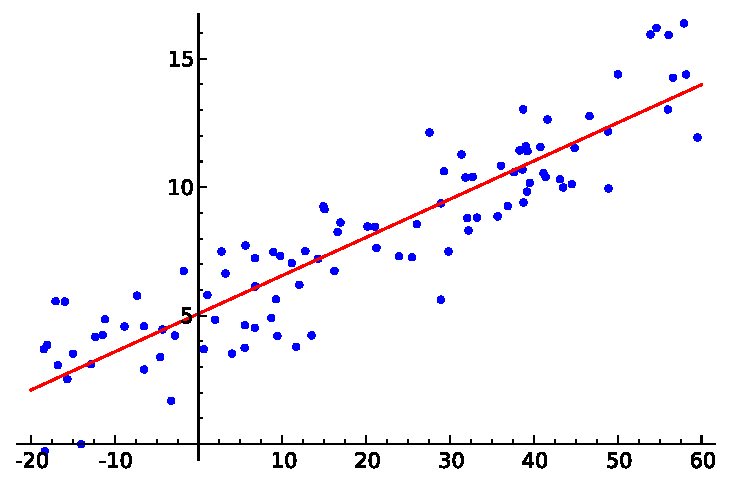
\includegraphics[width=0.5\linewidth]{figs/Linear_regression}
\caption{Linear regression of data}
\end{figure}
Given a vector of inputs \(X^T=(X_1,\ldots,X_d)\). The output variable (also called response variable) is predicted via the model\\
\[Y = \beta_0 + \sum^d_{j=1} X_j\beta_j,~~ Y \in \R\]
\(\beta_0\) is called bias(Machine Learning) or intercept (Statistics). We extend the X vector with an \(X_0 = 1\) and we can include the bias \(\beta_0\) into the vector of \(\beta\)s and can write Y in matrix form: \(Y = X^T\beta,~~X,\beta \in \R^{d+1}\)
\subsubsection{Training of the Linear Regressor: Residual Sum of Squares(RSS)}
Training of an accurate Predictor = Minimize the residual sum of squares between the actual value \(y\) and the predicted \(\overline{X}\beta\):\\
\[RSS(\beta) = \sum^{n}_{i=1}(y_i-x_i^T\beta)^2\] or matrix notation \[RSS(\beta) = (y-\overline{X}\beta)^T(y-\overline{X}\beta),~~X\in \R^n \times \R^{d+1}\] \(\text{(Each row of } \overline{X} \text{ is an input vector } X, y \text{ is an n-vector of the outputs in the training set})\)\\\\
We find the minimum RSS by differentiating w.r.t. \(\beta\)\\ 
\begin{align}
&\rightarrow X^T(y-X\beta) = 0\\
&\rightarrow\hat{\beta} = (X^TX))^{-1}X^Ty~~(\text{Solution for nonsingular} X^TX)
\end{align}
\subsubsection{Prediction via the Trained Linear Regressor}
\[\hat{y} = X \hat{\beta} = X(X^T X)^{-1} X^T y\]
The matrix \(X(X^T X)^{-1} X^T\) is sometimes called the hat matrix
which is an orthogonal projection on the space spanned by the columns of X.
\subsubsection{Perturbation of Linear Regressor with Gaussian Noise}
Gaussian noise \(\epsilon\) with \(\mathcal{E}(\epsilon) = 0, \mathcal{V} = \sigma^2\)
\begin{proof}
\begin{align}
Y &= \E(Y|X_1 , \ldots , X_d) + \epsilon\\
&= \beta_0 + \sum^d_{j=1} X_j \beta_j + \epsilon\\
&= X\beta + \epsilon
\end{align}
Meaning that gaussian noise does not perturb the estimator.
\end{proof}

\subsubsection{Optimality of Least Squares Estimate}
The least squares estimate of the parameter \(\beta\) has the smallest variance among all linear unbiased estimates.\\
We want to predict a. Prediction \(\hat{\theta}\) is a linear function \(c_0^Ty = \overbrace{a^T (X^T X)^{-1} X^T}^{c_0} y\) of the response vector y.
\begin{proof}

\(a^T \hat{\beta}\) is unbiased since the expectation \(\E\) yields
\begin{align}
\E(a^T \hat{\beta}) &= \E(a^T (X^T X)^{-1} X^T y)\\
&= a^T (X^T X)^{-1} X^T \E(X\beta + \epsilon)\\
&= a^T (X^T X)^{-1} X^T (X\beta + \underbrace{\E(\epsilon)}_{=0} ) = a^T \beta\\
\end{align}
Variance of \(a^T\hat{\beta}\)
\begin{align}
\V(a^T \hat{\beta}) &= \V\Big( a^T \underbrace{(X^T X)^{-1} X^T \overbrace{(X\beta + \epsilon)}^{y}}_{\hat{\beta}}\Big)\\
&= \underbrace{\V(a^T \beta)}_{=0} +\V\left(a^T (X^T X)^{-1} X^T \epsilon\epsilon^T X(X^T X)^{-1} a\right)
= \sigma^2 a (X^T X)^{-1} a
\end{align}
The cross-correlations are linear in \(\epsilon\) and, therefore, they vanish.\\\\
Alternative unbiased linear estimator (to show the least squares estimator is the best)
\begin{align}
\hat{\theta} &= c^T y = a^T \hat{\beta} + a^T Dy\\
\E(c^T y) &= \E(a^T \hat{\beta}) + \E(a^T Dy) = a^T \beta + \E a^T D(X\beta + \epsilon)\\
&= a^T \beta + a^T DX\beta + a^T D \underbrace{\E(\epsilon)}_{=0} = a^T \beta\\
\end{align}
The (unbiasedness) condition \(\E(c^T y) = a^T \beta\) implies \(DX = 0\).
\end{proof}
Gauss-Markov Theorem proves \(\V(a^T\hat{\beta}) \leq \V(c^Ty)\) (The least squares estimator is the best unbiased linear estimator)
\subsection{Ridge Regression}
Ridge regression is a regularized version of the linear regression with the same closed form but adds a penalty term to it to restrict the solution. It still has a closed solution, but now depends on the \(\lambda\) parameter. The \(\lambda\) shrinks the regression coefficients by imposing a penalty on their size. This is done via a cost function:
\[\hat{\beta}^{ridge} = \argmin_{\beta} \Big\{\sum^{n}_{i=1}(y_i - \beta_0-\sum^d_{j=1}x_{i,j}\beta_j)^2+\underbrace{\lambda \sum^d_{j=1} \beta^2}_{L_2 \text{ norm penalty}}\Big\}\]
\(\lambda \leq 0\) controls the amount of shrinkage (Weight decay in Neuronal Network Literature). The penalty term is \(\lambda\) times the \(L_2\) norm (\hyperref[Norms@Glossary]{Norms@Glossary}), which is the Euclidian length of the \(\beta\) vector. \\
\url{https://en.wikipedia.org/wiki/Tikhonov_regularization}
\subsubsection{Solution to Ridge Regression}
Shift the coordinate system into the center of mass of the data distribution:
\[x_{i,j} = x_{i,j}-\overline{x}_{j},\beta_0 = \sum^n_{i=1} \frac{y_i}{n}\]
By this, we reduce the system from d+1 to d dimensions (\hyperref[homogeneous-coordinates@Glossary]{homogeneous coordinates@Glossary}) and get:\\
\[RSS(\beta) = (y-X\beta)^T(y-X\beta)+\lambda\beta^T\beta\]
The ridge solution is then:
\[\hat{\beta}^{ridge} = \underbrace{(X^T X + \lambda I)^{-1}}_{X^T X\text{ is regularized by }\lambda I}X^Ty\]
This can also be solved via Singular value decomposition (\hyperref[SVD@Glossary]{SVD@Glossary}).
\subsection{The LASSO}
An alternative regularized version of least squares is LASSO (Least absolute shrinkage and selection operator). It uses the same unconstrained linear regression with the same closed form but add a penalty term to it to restrict the solution, as it is done in the ridge regression. \[\hat{\beta}^{LASSO} = \argmin_{\beta} \Big\{\sum^{n}_{i=1}(y_i - \beta_0-\sum^d_{j=1}x_{i,j}\beta_j)^2\Big\}\] subject to \[\sum^{d}_{j=1}|\beta_j| \leq s\] The lower equation is the penalty term, which is different from the ridge regression and is the \(L_1\) norm penalty, which is the so-called ''Manhattan distance'' (\hyperref[Norms@Glossary]{Norms@Glossary}). The LASSO does not have a closed form anymore and must must be solved numerically by using quadratic programming or more general convex optimization methods.\\
\url{https://en.wikipedia.org/wiki/Least_squares#Lasso_method}
\subsubsection{Ridge vs. LASSO Estimation}
One of the prime differences between LASSO and ridge regression is that in ridge regression, as the penalty is increased, all parameters are reduced while still remaining non-zero, while in LASSO, increasing the penalty will cause more and more of the parameters to be driven to zero. This is an advantage of LASSO over ridge regression, as driving parameters to zero deselects the features from the regression. Thus, Lasso automatically selects more relevant features and discards the others, whereas Ridge regression never fully discards any features.
\begin{figure}[H]
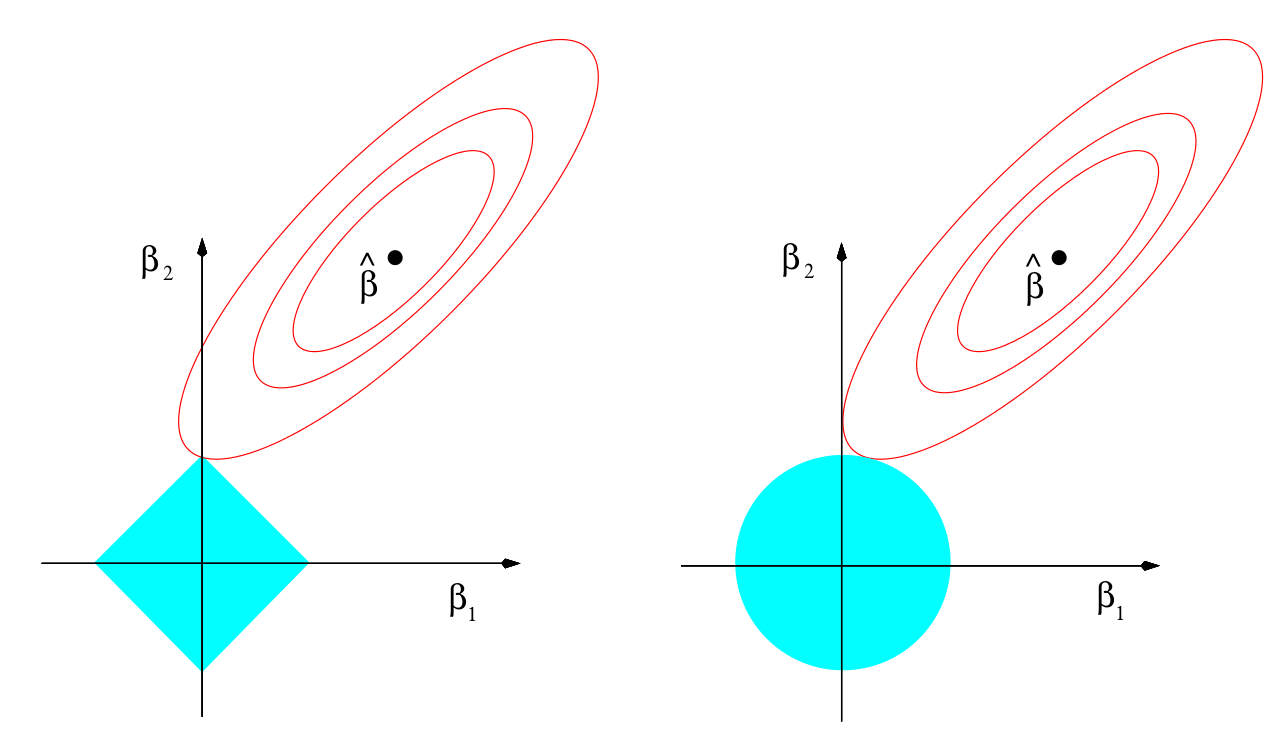
\includegraphics[width=\linewidth]{figs/LASSO-vs-Ridge}
\caption{Estimation picture for the LASSO (left) and Ridge regression (right). Shown are contours of the least squares error function (red) and constraint functions \(|\beta_1 | + |\beta_2 | \leq t\) and \(\beta_1^2 + \beta_2^2 \leq t_2\) (blue). Therefore LASSO estimates are known to zero-out several coefficients and only keep a few non-zero. The reason is that the LSE error surface often hits the corners of the constraint surface(Source: fig 3.12 of Hastie et al. 2001)}
\end{figure}
\subsubsection{Generalized Ridge Regression}
The generalized ridge regression has known closed forms for certain values of \(p\).
\[\hat{\beta}^{ridge} = \argmin_{\beta} \Big\{\sum^{n}_{i=1}(y_i - \beta_0-\sum^d_{j=1}x_{i,j}\beta_j)^2+\underbrace{\lambda \sum^d_{j=1} |\beta|^p}_{L_P \text{ norm penalty}}\Big\}\]
For \(p = 2\), we get the usual Ridge Regression with the closed form as described above. For \(p = 1\), we get the LASSO Regression as described above and for all other values we get regression with different strengths of shrinkage as shown below.

\begin{figure}[H]
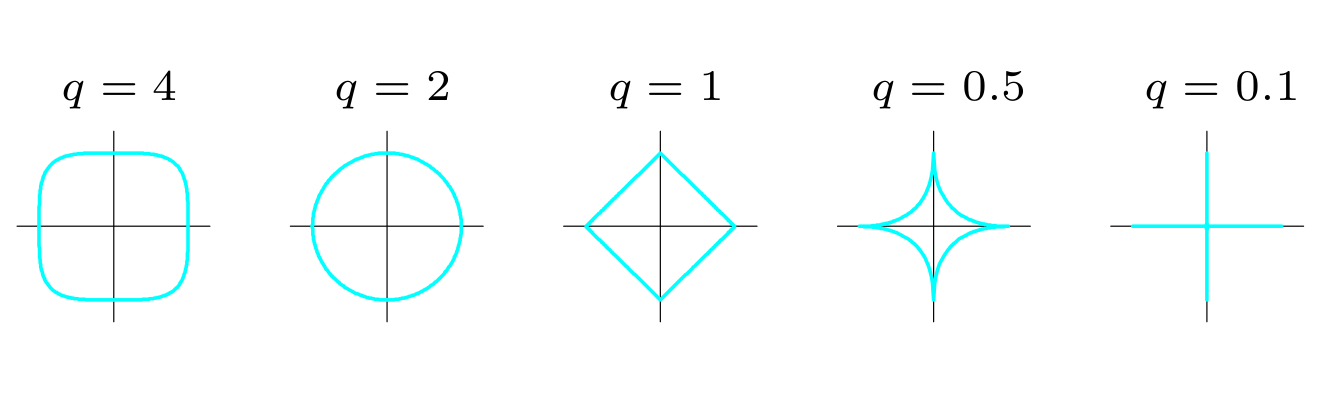
\includegraphics[width=\linewidth]{figs/different-strengths-of-shrinkage}
\caption{Contours of constraint functions \(\sum_{j}|\beta_j|^p\) for different values of \(q\) (Source: HTF'01)}
\end{figure}

\subsection{Nonlinear Regression by basis expansion}
Idea: Transform the variables X nonlinearly and fit a linear model into the resulting (feature) space. Transformation: \(h_m(X) : \R^d \rightarrow \R, 1 \leq m \leq M\)
\[f(X) = \sum^M_{m=1} \beta_m h_m(X)\]
f is linear in \(\beta\) but non-linear in X! We use a series of piecewise-cubic polynomials to fit the data, of which the smoothness can be controlled by regularization of the the maximal number of knots.
\subsection{Wavelet regression}
Regression can also be done with Wavelets. A wavelet is a wave-like oscillation with an amplitude that begins at zero, increases, and then decreases back to zero. It can typically be visualized as a ''brief oscillation'' like one might see recorded by a seismograph or heart monitor. Generally, wavelets are purposefully crafted to have specific properties that make them useful for signal processing. Wavelets can be combined, using a ''reverse, shift, multiply and integrate'' technique called convolution, with portions of a known signal to extract information from the unknown signal. (Source: Wikipedia.org)
\begin{figure}[H]
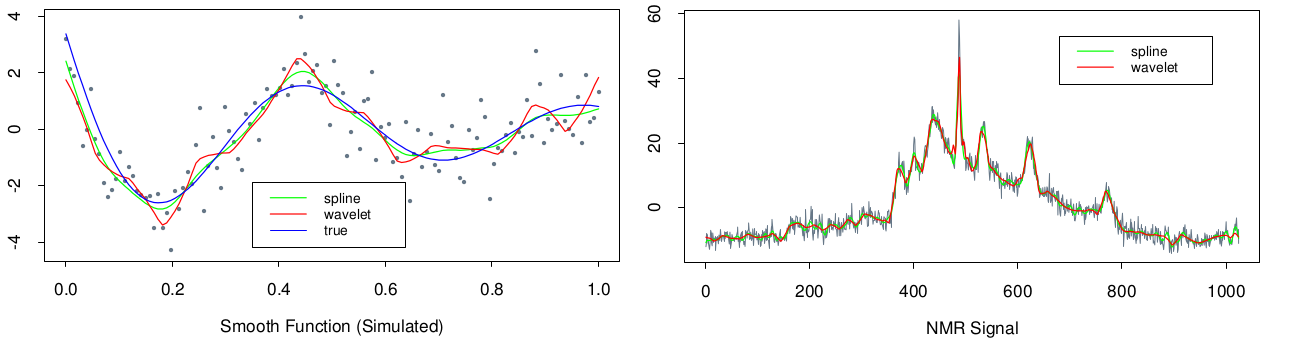
\includegraphics[width=\linewidth]{figs/Wavelet-vs-Spline}
\caption{Wavelet smoothing compared with smoothing splines on two examples. Each panel compares the SURE-shrunk wavelet fit to the crossvalidated smoothing spline fit. (Source: HTF'01)}
\end{figure}
\subsection{Bias-variance-Tradeoff in Regression}
We have data \(D = \{(x_i,y_i)\}^n_{i=1},~~x_i \in \R^d,y_i \in \R\) which contains observations of the random variables \((X_i,Y_i)\) which are drawn i.i.d. from the distribution \(P(X,Y)\). We have the objective to find a regression function \(f \in \mathcal{F}\)(\(\mathcal{F}\) is the hypothesis class) such that \(\E(Y - f(X))^2\) is minimal. We can find the optimum at \(f^*(x) = \E(Y|X = x)\). So we construct an estimator \(\hat{f}(X)\) which estimates Y depending on the random variable \(X\) and on the data \(D\).\\\\
\textbf{Problems resulting in the Tradeoff}
\begin{enumerate}
\item Finite training set
\item Complexity of hypothesis class \(\mathcal{F}\) is unknown
\end{enumerate}
So we must find the best balance between a complex \(\mathcal{F}\) (by overfitting which keeps the variance high) and simple \(\mathcal{F}\) (by underfitting which keeps the bias high). This can be done by minimizing the error components:\\
\begin{align}
\E_D\E_{X,Y}\left(\hat{f}(X)-Y\right)^2 
&= \E_D\E_X\left(\hat{f}(X) - \E(Y|X)\right)^2 + \E_{X,Y}\left(Y - \E(Y|X)\right)^2\\
&= \underbrace{\E_X \E_D\left(\hat{f}(X) - \E_D(\hat{f}(X))\right)^2}_{variance} + \underbrace{\E_X\left(\E_D(\hat{f}(X)) - \E(Y|X)\right)^2}_{\text{bias}^2} + \underbrace{\E_{X,Y}\left(Y - \E(Y|X)\right)^2}_{\text{noise}}
\end{align}

Usually, it is very complex to minimize them both at the same time. 

\subsubsection{Combining regressors}
\paragraph{Bias}
A set of unbiased estimators that is simply averaged remains unbiased after averaging.
\[bias[f(x)] = \E_D\hat{f}(x) - \E(Y|x) = \frac{1}{B} \sum^B_{i=1}\E_D \hat{f}_i(x) - \E(Y|x) = \frac{1}{B} \sum^B_{i=1} \left(\E_D \hat{f}_i(x) - \E(Y|x)\right) =
\frac{1}{B} \sum^B_{i=1} bias[f_i (x)]\]
\paragraph{Variance}
\begin{align}
\V\{ \hat{f}(x)\} &= \E_D \hat{f}(X) - \E_D \hat{f}(X)
= \E_D(\frac{1}{B} \sum^B_{i=1} \hat{f}_i(x) - \frac{1}{B} \sum^B_{i=1} \E_D \hat{f}_i(x))^2\\
&= \E_D(\frac{1}{B} \sum^B_{i=1} (\hat{f}_i(x) - \E_D \hat{f}_i(x)))^2
= \frac{1}{B^2} \sum^B_{i=1} \V \{\hat{f}_i(x)\} + \frac{1}{B^2} \sum_{i\neq j}\sum \C ov\{\hat{f}_i(x),\hat{f}_j(x)\}
\end{align}
Assuming that covariances are small \(\C ov\{\hat{f}_i\} \approx 0\) and variances small as well \(\V\{\hat{f}(x)\} \approx \sigma^2\) then we can reduce to \(\V\{\hat{f}(x)\} \approx \frac{\sigma^2}{B}\). So the variance reduces by \(\frac{1}{B}\) if bias remains the unchanged.
\end{document}